\documentclass[12pt,a4paper]{article}
\usepackage[left=2.5cm,top=2.5cm,right=2.5cm,bottom=2.5cm,nofoot]{geometry}
\pagestyle{myheadings}
  
\usepackage[utf8]{inputenc}      

%Egna paket
\usepackage[swedish]{babel}
\usepackage[locale=DE, separate-uncertainty=true, multi-part-units=single]{siunitx}
\usepackage{amsmath, gensymb, array, siunitx}
\usepackage{graphicx, float, pgf, subcaption}
\graphicspath{{./images/}}
\usepackage{csvsimple, longtable, booktabs, listings}
\usepackage{enumitem}
\usepackage{blindtext, comment}
\usepackage{hyperref, csquotes}
\hypersetup{hidelinks}

\usepackage[style=ieee]{biblatex}
\addbibresource{references.bib}

\markright{Oskar Jonsson \& Vidar Petersson, Grupp 16, Uppgift 4}

\begin{document}
\pagenumbering{gobble} 

\begin{center}
    \vspace*{0.8cm}
    {\huge\bf STÖTAR \& ÖVERFÖRING}\\
    \vspace{0.5cm}
    \large{Rapport gällande faktorer som påverkar elasticitet, energibevaring och rörelsemängdsmomentsöverföring i stötar.}\\
\end{center}
\vspace{1.0cm}

\begin{center}
Oskar Jonsson (cid: osjon) och Vidar Petersson (cid: vidarp)

Program: Teknisk Fysik. 

Kurs: Experimentell fysik 1 - mätteknik, TIF083, del A.
\end{center}
\vspace{1.0cm}

\centerline{\bf Sammandrag}
\noindent Denna rapport undersöker kollisioner i en och två dimensioner med fokus på bevarande och fördelning av energi och rörelsemängd samt rörelsemängdsöverföring. I endimensionella kollisioner av ryttare på en luftskena studeras sambandet mellan stötkoefficienten $e$ och den relativa kollisionshastigheten $v_{\text{rel}}$ för olika material. Resultaten visar att $e$ minskar när $v_{\text{rel}}$ ökar, med olika karaktär beroende på material. I tvådimensionella kollisioner för puckar på ett luftbord analyseras påverkan av kollisionspunkten $d$ mellan två puckar för fördelningen av kinetisk energi, rörelsemängd och rörelsemängdsmomentsöverföring. Resultaten avslöjar att fördelningen av kinetisk energi förändras avsevärt med $d$, med en ökning av andelen rotationsenergi när $d$ ökar. Dessutom analyseras riktningen på rörelsemängden efter kollisionen i förhållande till kollisionspunkt $d$. Resultaten ger värdefulla insikter om energi- och rörelsemängdsbevarande i olika dimensioner och har implikationer för tillämpningar som kollisionssimuleringar och beräkningar av planetsystem. Rapporten belyser även vikten av att beakta faktorer som friktion i riktiga kollisionssituationer, vilket kan avvika från idealiska teoretiska modeller.

{\bf Nyckelord:} kollision, stötkoefficient, energibevaring, elasticitetsgräns


\centerline{\bf Abstract}
\noindent This report investigates collisions in one and two dimensions with a focus on the conservation and distribution of energy and momentum, as well as momentum transfer. In one-dimensional collisions of riders on an air track, the relationship between the coefficient of restitution $e$ and the relative collision velocity $v_{\text{rel}}$ for different materials is studied. The results show that $e$ decreases as $v_{\text{rel}}$ increases, with different characteristics depending on the material. In two-dimensional collisions of pucks on an air table, the impact of the collision point $d$ between two pucks on the distribution of kinetic energy, momentum, and angular momentum transfer is analyzed. The results reveal that the distribution of kinetic energy changes significantly with $d$, with an increase in the proportion of rotational energy as $d$ increases. Additionally, the direction of momentum after the collision in relation to the collision point $d$ is analyzed. The results provide valuable insights into the conservation of energy and momentum in different dimensions and have implications for applications such as collision simulations and calculations of planetary systems. The report also highlights the importance of considering factors like friction in real collision situations, which may deviate from ideal theoretical models.

{\bf Key words:} collision, coefficient of restitution, conservation of energy, elastic limit


\newpage

\tableofcontents
\newpage

\pagenumbering{arabic} 
\section{Inledning}
Stöt, eller kollision, är ett fenomen inom klassisk mekanik där kroppar möts och växelverkar under kort tid. Dessa stötar sker i allt från galaxer ner till den mikroskopiska nivån. Därför är det intressant att undersöka hur olika ingående faktorer påverkar stötars egenskaper. Detta arbete syftar speciellt till att presentera hur bevaring och överföring för stötar i olika dimensioner påverkas.

Det övergripande målet med detta arbete är att analysera energi- och rörelsemängds-bevaring för stötar i en och två dimensioner samt rörelsemängdsmomentöverföring i två dimensioner. För att uppfylla detta mål koncentrerar sig detta arbete på att besvara följande två konkretiserade frågeställningar:

\begin{itemize}
    \item Hur påverkar relativ kollisionshastighet för olika material stötkoefficienten i en endimensionell stöt? %Rörelsemängd
    \item Hur påverkar kollisionspunkten mellan två puckar fördelningen av rörelsemängd, translations- och rotationsenergi samt rörelsemängdsmomentsöverföring i en två-dimensionell stöt?
\end{itemize}

Genom en kombination av teoretisk analys, experimentell datainhämtning och dataanalys syftar vi till att ge insikter av betydelse inom ovanstående faktorer som styr kollisioner. Dessa insikter kommer att vara av betydelse för tillämpningar inom olika fysikaliska och tekniska områden som till exempel krocksimulationer och beräkning av planetsystem.

\begin{comment}
    Här beskriver du vad laborationen går ut på, helt enkelt vad den syftar till att göra. Detta gör du för att 
(i) förbereda läsarna på resten av rapporten på ett bra sätt (ii) hjälpa läsarna att förstå på vilket sätt de 
bör läsa rapporten (så att de läser den som du vill/d. v. s. läser den på ”rätt sätt”), och för att (iii) läsarna 
ska kunna använda det som sägs här som ett slags färdriktningsvisare för läsningen av rapporten (läsare 
av den här typen av texter gillar att du skapar, och infriar, förväntningar).   
Skriv  gärna  det  här  avsnittet  i  rapporten  enligt  ett  deduktivt  mönster;  inled  med  något  generellt 
påstående, men naturligtvis ett påstående med direkt koppling till det som ska göras, t. ex. ”Då en kropp 
faller från vila påverkas den i huvudsak av två krafter”, eller något liknande. Succesivt ska texten röra 
sig från det generella till det specifika, d. v. s. syftet med undersökningen/laborationen.  
Syftet anges ibland i instruktionerna till en (lärande)laboration och då är det naturligt att använda något 
liknande den beskrivningen. I ”verklighetens” rapporter finns det sällan instruktioner för en laboration 
och då är det viktigt att man formulerar syftet med laborationen på ett mycket tydligt sätt för läsarna – i 
annat fall riskerar man att de helt missar det som rapporten är tänkt att göra; akademiska texter är texter 
som ARBETAR, texter som GÖR något för läsaren. 
\end{comment}

\section{Teori} \label{sec:teori}
Kollisioner mellan kroppar introducerar överföring av rörelsemängd, rörelsemängdsmoment och energi som är centrala inom den klassiska mekaniken. Dessa fenomen beskriver förändring av kroppars translation och rotation i deras rörelsedimensioner och är bevarade ur ett systemspecifikt perspektiv, det vill säga att dessa kroppars förändring av dessa storheter går att förutspå med hjälp av uttryck härledda från Newtons lagar. 

Rörelsemängd är en vektorstorhet, betecknat $\mathbf{p}$, som är vektorprodukten av en kropps massa \emph{m} och dess hastighetsvektor $\mathbf{v}$. Rörelsemängden är bevarad i ett slutet system om inga yttre impulser påverkar systemet vilket innebär att ett system av flera kroppars rörelsemängd kan adderas med avseende på varje kropps enskilda rörelsemängd enligt \cite{Meriam_Kraige_Bolton_2020} %Rätt ställe?

\begin{equation} \label{rörelsemängd}
    \mathbf{p}= \sum_i m_i\mathbf{v}_i\text.
\end{equation}

Rörelsemängdsmoment är även det en vektorstorhet som beskriver en kropps rotationstillstånd med avseende på dess massfördelning samt vinkelhastighet. Denna storhet beskrivs generellt med uttrycket

\begin{equation} \label{rörelsemängdsmoment}
    \mathbf{L}_{O}   = \bar{\mathbf{I}}\boldsymbol{\omega} + \mathbf{r}_{MC} \times \mathbf{p}
\end{equation}

där $\mathbf{L}_{O}$ är rörelsemängdsmomentet kring en godtycklig punkt i systemet, $\mathbf{r}_{MC}$ är ortsvektorn till kroppens masscentrum och $\mathbf{p}$ är kroppens rörelsemängdsvektor. $\bar{\mathbf{I}}$ är kroppens tröghetsmoment med avseende på masscentrum och $\boldsymbol{\omega}$ är kroppens rotationsvektor med avseende på masscentrum. Rörelsemängdsmoment är likt rörelsemängden bevarad i ett slutet system \cite{Meriam_Kraige_Bolton_2020}. Vid analys av enbart rörelsemängdsmoment kring masscentrum kan den förenklade formeln $\mathbf{L}_{MC} = \bar{\mathbf{I}}\boldsymbol{\omega}$ användas. 

Den totala kinetiska energin för en kropp definieras enligt
 \begin{equation}\label{kinetiskenergi}
     T_{\text{tot}} = T_{\text{trans}}+T_{\text{rot}} = \frac{1}{2}mv^2 + \frac{1}{2}\Bar{I}\omega^2
 \end{equation}
där parametrarna är de storheter som tidigare definierats i ekvation \eqref{rörelsemängd} och \eqref{rörelsemängdsmoment} för en godtycklig kropp fast utan sina vektoregenskaper vilket leder till att $T$ inte har någon riktning utan enbart är en skalär \cite{Meriam_Kraige_Bolton_2020}.

I ett slutet system är energin enbart bevarad i idealfallet. Detta innebär att i en ideal stöt mellan två kroppar är den totala energi för systemet konstant. I praktiken är en stöt däremot oftast inelastisk och en energiförlust sker på grund av exempelvis plastisk deformation, värme eller ljud. Elasticiteten för en endimensionell stöt beskrivs av stötkoefficienten enligt 
\begin{equation} \label{ekv:e}
     e = \frac{v_{\text{rel}}'}{v_{\text{rel}}}
 \end{equation}
där $v_{\text{rel}}'$ är relativa hastigheten omedelbart efter och $v_{\text{rel}}$ omedelbart före kollision. Stöt-koefficient med kvot 1 representerar således en perfekt elastisk stöt. I allmänhet betraktas $e$ för stöt mellan två kroppar som en konstant beroende på deras material \cite{Meriam_Kraige_Bolton_2020}. Dock visar en mer rigorös analys att även kollisionshastighet påverkar $e$ \cite{stöte}. För hårda material bestämmer deras elasticitetsgräns den högsta spänning de tål utan att deformeras plastiskt. För små kollisionshastigheter är spänningarna i materialet under elasticitetsgränsen och således uppträder materialet helt elastiskt i likhet med en fjäder och all energi bevaras. Om spänningarna däremot överstiger elasticitetsgränsen kommer enbart en del av energi bevaras, resten förloras till deformation. I kollisioner är impulsen i materialet proportionerligt med $v$. Teoretiskt konvergerar därför $e$ för alla material i 1 för små kollisionshastigheter \cite{Meriam_Kraige_Bolton_2020}. 




%Genom att studera bevarandet av dessa storheter i ett slutet system kan man med hjälp av de uttryck som presenterats bestämma överföringen av rörelsemängd, rörelsemängdsmoment samt energi för kropparna i systemet. Denna teori är därmed essentiell för att studera stötkoefficienten, fördelningen mellan rörelsemängd och rörelsemängdsmoment samt energibevaringen för två kroppar i ett slutet system.



\section{Metod}
Den experimentella datainsamlingen bestod av två olika uppställningar för att tillsammans svara på de två respektive frågeställningarna. I del 1 undersöktes stötar i en dimension och deras stötkoefficient. I del 2 utvidgades undersökningen till två dimensioner och även fördelning av energi, rörelsemängd och rörelsemängdsmoment i två dimensioner undersöktes. Nedan redovisas det material, uppställningar och tillvägagångssätt som användes.

\subsection{Material och uppställning} 

För del 1 användes ryttare av metall på en luftskena för att modellera endimensionella stötar, enligt figur \ref{fig:del1}. Luftskenan var av modell Pasco physics airtrack (SF-9214) och var hopkopplad med en luftfläkt av modell Frederiksen Air Blower 1970,70. Ovanpå själva ryttarna som gled längs luftskenan placerades två metallvikter och reflextejp för att mäta ryttarnas position med ett kamerasystem. De extra vikterna placerades på toppen i syfte att förskjuta masscentrum uppåt och därmed minska impulsmomentet i stötarna och således motverka oönskad rörelse i $\hat z$-led. I den ena mätserien försågs även en av ryttarna med en anordning beståendes av en klyka med gummiband. Detta för att undersöka hur materialet i kollisionspunkten påverkar stötkoefficienten.

\begin{figure}[H]
    \centering
    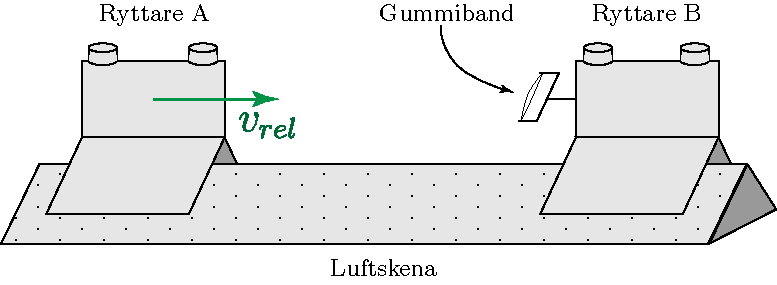
\includegraphics[width=0.8\linewidth]{images/metod/ryttare.pdf}
    \caption{Försöksuppställningen för endimensionella stötar. Två ryttare på en luftskena kolliderade med relativ hastighet $v_{\text{rel}}$. I första mätserien utgjordes deras kontaktpunkt av ett uppspänt gummiband. I den andra skedde kollisionen metall mot metall.}
    \label{fig:del1}
\end{figure}

 För del 2 användes istället ett luftbord med två metallpuckar, enligt figur \ref{fig:del2}, för att undersöka stötar i två dimensioner. Luftbordet kopplades i sin tur till samma luftfläkt som i del 1. Utanpå puck A placerades ett gummiband i syfte att öka friktionen mellan kontaktytorna vid stötarna. Ovanpå vardera puck placerades även tre bitar reflextejp för att mäta position och rotation. Bitarna placerades på randen för att möjliggöra numerisk beräkning av masscentrums translation och rotation med hög precision.
 
 Utöver utrustningen för respektive uppställningen användes även ett motion capture system från {Qualisys} av modell Oqus 300 monterat i taket för att mäta objektens position över tid med upplösning \(\SI{e-6}{m}\). Kamerasystemets uppdateringsfrekvsens valdes till 500 Hz för att erhålla högre upplösning i tid och med större noggrannhet bestämma kollisionsögonblicket.

\begin{figure}[H]
    \centering
    \begin{subfigure}{.5\textwidth}
        \centering
        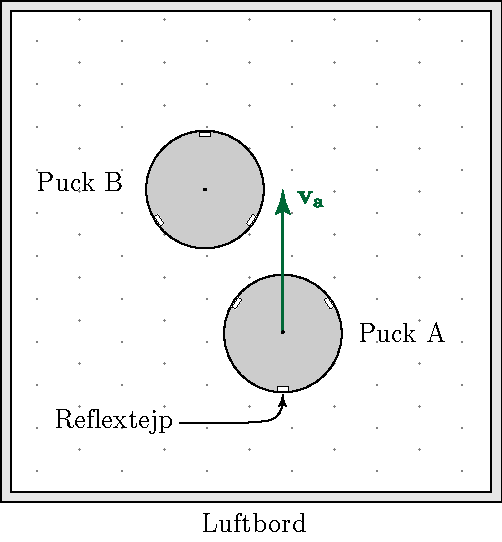
\includegraphics[width=0.95\linewidth]{images/metod/del2_bord.pdf}
        \caption{Uppställningen för de tvådimensionella stötarna av puckar på luftbord. Puck A kolliderade med initialhastighet $v_a$ i puck B. Längs puckarnas rander placerades reflextejp.}
        \label{fig:del2_bord}
    \end{subfigure} 
    \hfill
    \begin{subfigure}{.45\textwidth}
        \centering
        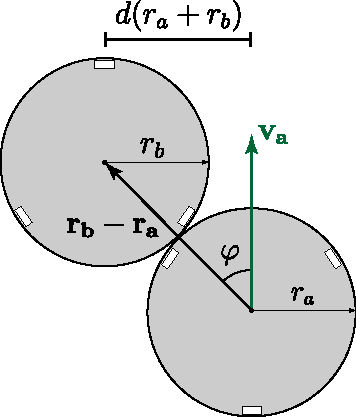
\includegraphics[width=0.75\linewidth]{images/metod/del2_kollision.pdf}
        \caption{Kollisionsparametrar för puckarna. Utskrivna är den icke-normaliserade kollisionspunkten $d(r_a+r_b)$, hastighetsvektorn $v_a$, ortsvektorn mellan masscentran $\mathbf{r_b}-\mathbf{r_a}$, relativa vinkeln $\varphi$ och radierna $r_a$ och $r_b$.}
        \label{fig:del2_collision}
    \end{subfigure}
    \caption{Försöksuppställning för de tvådimensionella stötarna på luftbordet sedd ovanifrån och deras kollisionsparametrar.}
    \label{fig:del2}
\end{figure}

\subsection{Genomförande} \label{chap:material}
Innan mätningarna genomfördes kalibrerades bordets och skenans lutning samt deras lufttillförsel för att minimera icke önskvärd energipåverkan i systemet. Konktaktytor torkades sedan av med desinfektionsdukar för att avlägsna ytbeläggningar av smuts och tejprester. Även kamerasystemet kalibrerades med tillhörande kalibreringsutrustning tills en residual runt $\SI{2e-4}{m}$ erhölls. I både del 1 och 2 mättes objektens relevanta konstanter innan med mätutrustning från labbsalen, se tabell \ref{tab:mätutr.}. I del 1 mättes massorna och i del 2 mättes massorna och radierna, se tabell \ref{tab:prop1} och \ref{tab:prop2}.

I första mätserien för del 1 monterades klykan med gummiband på ryttare B. Därefter placerades de på luftskenan och skickades iväg för hand mot varandra drygt 50 gånger med godtyckligt varierad relativ hastighet. För varje stöt startades en ny mätning med kamerasystemets mjukvara, Qualisys Tracking Manager (QTM), som löpande registrerade ryttarnas position. I den andra mätserien genomfördes samma procedur efter att klykan monterats av så att ryttarnas metallsidor blev ny kontaktpunkt.  %Ev. förklara lika hastigheter

Utifrån den erhållna positionsdatan beräknades den relativa kollisionshastigheten $v_{\text{rel}}$ innan kollisionsögonlicket samt stötkoefficienten $e$ med datanalys i \textit{Python}, se listing \ref{lst:1main} i bilaga \ref{bil:kod}. Koefficienten beräknades genom att ta medelvärdet av $v_{\text{rel}}$ under 0,2 sekunder innan och efter stöten för att sedan dividera dem enligt ekvation \eqref{ekv:e}. %Ev förklara varför 0.2s

I del 2 placerades puckarna på luftbordet där puck A sköts för hand mot den stillastående pucken B. Detta skedde drygt 50 gånger där vinkel och träffpunkt varierades godtyckligt. Utifrån den insamlade positionsdatan från markörerna på randen beräknades initialt puckarnas masscentrums translation och rotation numeriskt, se bilaga \ref{bil:kod} tabell \ref{lst:2center_calc}. Utifrån det beräknades därefter puckarnas translationshastighet $\mathbf{v_i}$, vinkelhastighet $\omega_i$, rörelsemängd $\mathbf{p_i}$, rörelsemängdsmoment $\mathbf{L_{MC}}_i$ och kinetiska energi $T_i$ numeriskt enligt dataanalysen i bilaga \ref{bil:kod} och teorin i avsnitt \ref{sec:teori}. För att besvara frågeställningen om bevaring och fördelning innan och efter stöt studerades enbart medelvärdet av parametrarna 0,2 sekunder innan och efter kollisionstillfälle. Kollisionspunkten $d$ definierades däremot som det normerade avståndet mellan masscentran vinkelrät mot hastighetsvektorn i kollisionsögonblicket. Kvoten beräknades enligt 
\begin{equation} \label{ekv:d_calc}
    d=\frac{\sin(\varphi)||\mathbf{r_b}-\mathbf{r_a}||}{(r_a+r_b)}.
\end{equation} %Gör tydligare skillnad på orts och radier
utifrån parametrarna redovisade i figur \ref{fig:del2_collision}.

Innan varje mätserie påbörjades genomfördes även en referensmätning av påverkan från eventuell friktion och luftströmmar. Objekten sköts över kollisionsområdet på luftskenan respektive luftbordet för att sedan numeriskt beräkna påverkan. 

\section{Resultat}
Nedan presenteras resultaten för samtliga mätserier beskrivna i avsnitt \ref{chap:material} i form av figurer och regressionsanalyser. I varje mätserie registrerades drygt 50 mätpunkter där den relativa hastigheten $v_{\text{rel}}$ för ryttarna varierades i det endimensionella fallet och förhållandet mellan puckarnas centrum $d$ enligt ekvation \eqref{ekv:d_calc} i fallet med två dimensioner. Behandling av rådatan görs enligt dataanalys i bilaga \ref{bil:kod} för att få relevanta parametrar till figurerna. 

\subsection{En dimension}
I figur \ref{fig:endimstöt} presenteras mätserier för uppställning \ref{fig:del1}  där $v_{\text{rel}}$ varieras på x-axeln och den beräknade stötkoefficienten från ekvation \eqref{ekv:e} på y-axeln. I figur \ref{fig:estötgummi_bord} användes det gummbiband som visas i figur \ref{fig:del1} som kontaktpunkt vilket visar ett linjärt samband mellan $v_{\text{rel}}$ och $e$. Detta samband visas med hjälp av regressionslinjen $y = -0,24x + 0,89$ som har ett $R^2$-värde på 0,96. Figur \ref{fig:estötmetall} behandlar istället ryttarna utan gummibandet som kontaktpunkt vilket istället visar ett potenssamband enligt  regressionslinjen $y = 0,07x^{-0,42}$ som har ett $R^2$-värde på 0,93.


\begin{figure}[H]
    
    \begin{subfigure}{.5\textwidth}
        \centering
        \hspace*{-1.2cm}
        \includegraphics[width=1\linewidth]{images/estöt_gummi.pdf} %R-squared value: 0.9640957801029384
        \caption{Stötkoefficient beroende på $v_{\text{rel}}$ för ryttare med gummiband som kontaktpunkt.}
        \label{fig:estötgummi_bord}
    \end{subfigure} 
    \hfill
    \hspace*{0.2cm}
    \begin{subfigure}{.5\textwidth}
        \centering
        \hspace*{-1.2cm}
        \includegraphics[width=1\linewidth]{images/estöt_metall.pdf} %R-squared value: 0.9252747767277821
        \caption{Stötkoefficient beroende på $v_{\text{rel}}$ för ryttare med ryttarnas metall som kontaktpunkt.}
        \label{fig:estötmetall}
    \end{subfigure}
    \caption{Stötkoefficienter för kollisioner av ryttare i en dimension. Notera minskningen av $e$ i samband med att $v_{\text{rel}}$ ökar.}
    \label{fig:endimstöt}
\end{figure}

\subsection{Två dimensioner}
I figur \ref{fig:energifördl} visas fördelningen av rotation samt translationsenergi av den totala energin för systemet beroende av $d$, där $d$ är det normerade avståndet mellan masscentran vinkelrät mot hastighetsvektorn i kollisionsögonblicket, enligt uppställningen i figur \ref{fig:del2_bord}.  

\begin{figure}[H]
    \begin{subfigure}{.48\textwidth}
        \centering
        \hspace*{-1.2cm}
        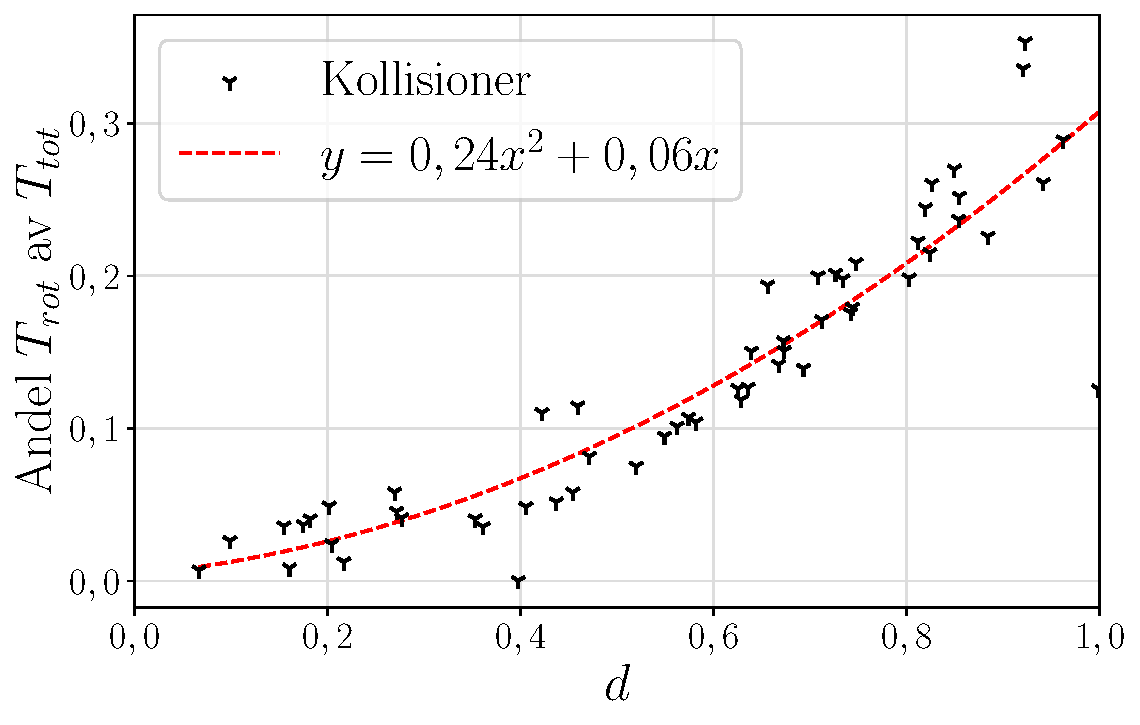
\includegraphics[width=1\linewidth]{images/d_rotationandel.pdf} %R-squared value: 0.8458396030717268
        \caption{Andel rotationsenergi av total energi för kollisioner mellan puckar i två dimensioner beroende på $d$.}
        \label{fig:rot}
    \end{subfigure} 
    \hfill
    \hspace*{0.2cm}
    \begin{subfigure}{.48\textwidth}
        \centering
        \hspace*{-1.2cm}
        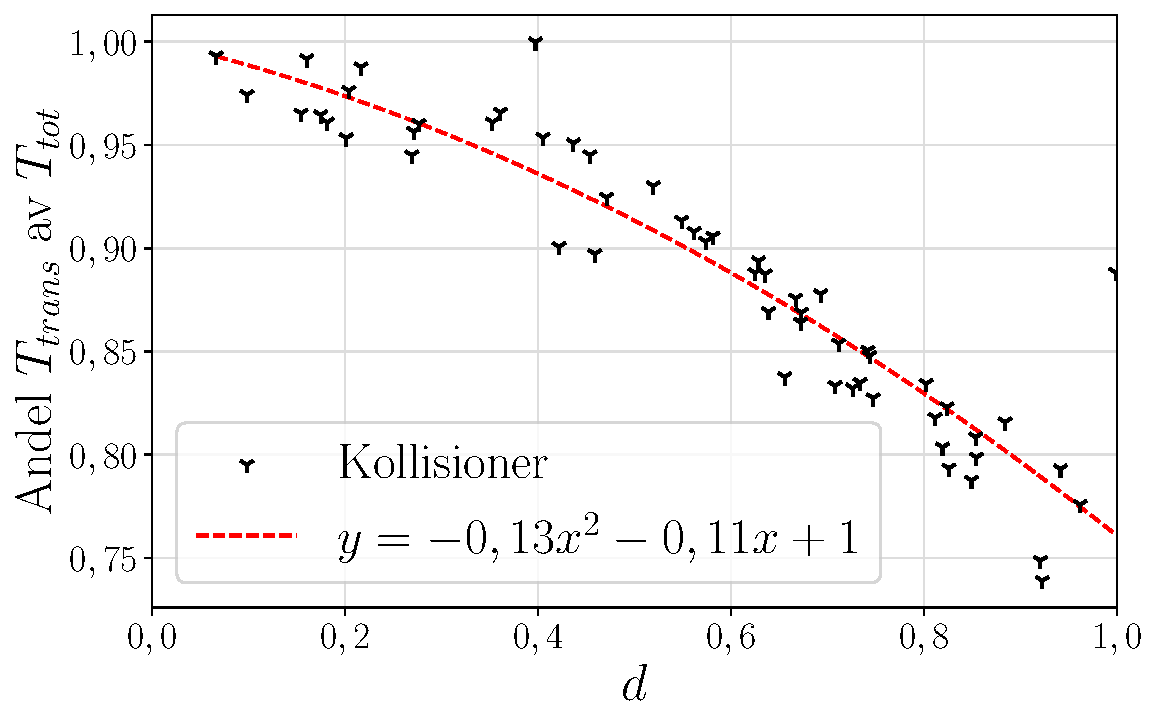
\includegraphics[width=1\linewidth]{images/d_translational_energy_percentage.pdf} %R-squared value: 0.8604999741824243
        \caption{Andel  translationsenergi av total energi för kollisioner mellan puckar i två dimensioner beroende på $d$.}
        \label{fig:trans}
    \end{subfigure}
    \caption{Andel rotations- och translationsenergi för två puckar med avseende på $d$. Notera sambandet mellan rotations- samt translationsenergi och $d$ genom figurernas motsatta trender. Regressionslinjerna har $R^2$-värde på 0,85 respektive 0,86.}
    \label{fig:energifördl}
\end{figure}

Med hjälp av både figur \ref{fig:rot} och figur \ref{fig:trans} syns sambandet att rotationsenergin för systemet ökar i samband med att $d$ ökar och att translationsenergin för systemet ökar när $d$ minskar.

I figur \ref{fig:rörelsemängd} visas rörelsemängden i x'-led och y'-led för puck B med avseende på hastighetsvektorn för puck A som nollställe i ett nydefinerat koordinatsystem med hastighetsvektorn för puck A som utgångspunkt.

\begin{figure}[H]
    
    \begin{subfigure}{.45\textwidth}
        \centering
        \hspace*{-1.2cm}
        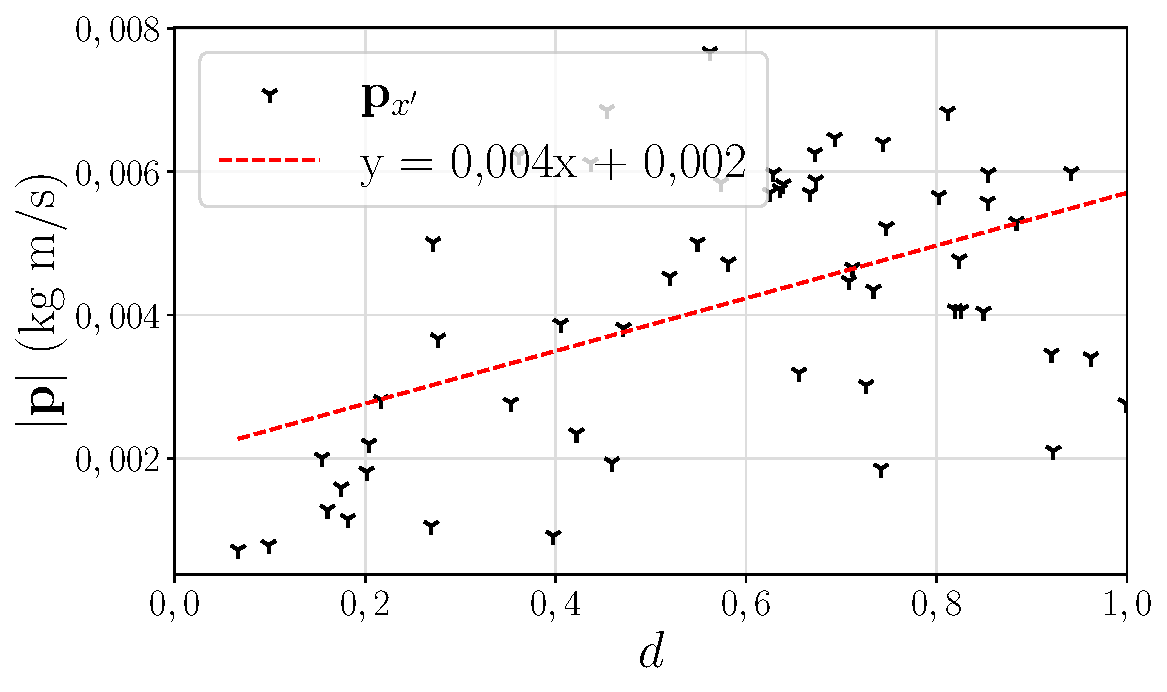
\includegraphics[width=1.2\linewidth]{images/d_pxled.pdf} %R-squared value: 0.2536796041858981
        \caption{Rörelsemängd för puck B i x'-led beroende av $d$. Notera sambandet mellan rörelsemängden och $d$.}
        \label{fig:px}
    \end{subfigure} 
    \hfill
    \begin{subfigure}{.45\textwidth}
        \centering
        \hspace*{-1.2cm}
        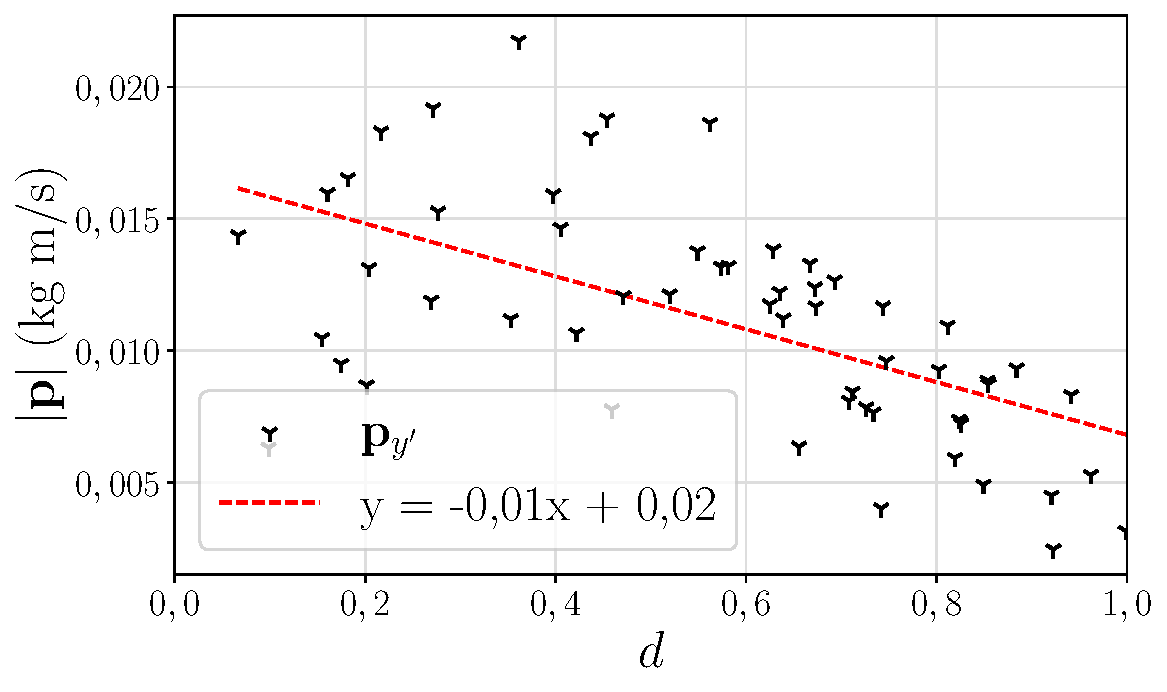
\includegraphics[width=1.2\linewidth]{images/d_pyled.pdf} %R-squared value: 0.34818806187610774
        \caption{Rörelsemängd för puck B i y'-led beroende av $d$. Notera sambandet mellan rörelsemängden och $d$.}
        \label{fig:py}
    \end{subfigure}
    \caption{Rörelsemängdskomposanter beroende av $d$ i ett nydefinerat koordinatsystem med puck A:s hastighetsvektor som utgångspunkt. Notera figurernas motsatta trender. Regressionslinjerna har $R^2$-värde på 0,25 respektive 0,35.}
    \label{fig:rörelsemängd}
\end{figure}
Med hjälp av figur \ref{fig:px} och figur \ref{fig:py} syns sambandet mellan rörelsemängden i x'-led och y'-led i relation till $d$.


I figur \ref{fig:lb-label} visas differensen för den absoluta rörelsemängden för hela systemet före och efter kollision beroende av $d$ där många punkter är centrerade runt 0. I figur \ref{fig:lb-label} visas istället det absoluta rörelsemängdsmomentet för puck B beroende av $d$ där det syns att $\mathbf{L}_b$ ökar i samband med att $d$ ökar. 
 

\begin{figure}[H]
    
    \begin{minipage}{.45\textwidth}
        \centering
        \hspace*{-1.2cm}
        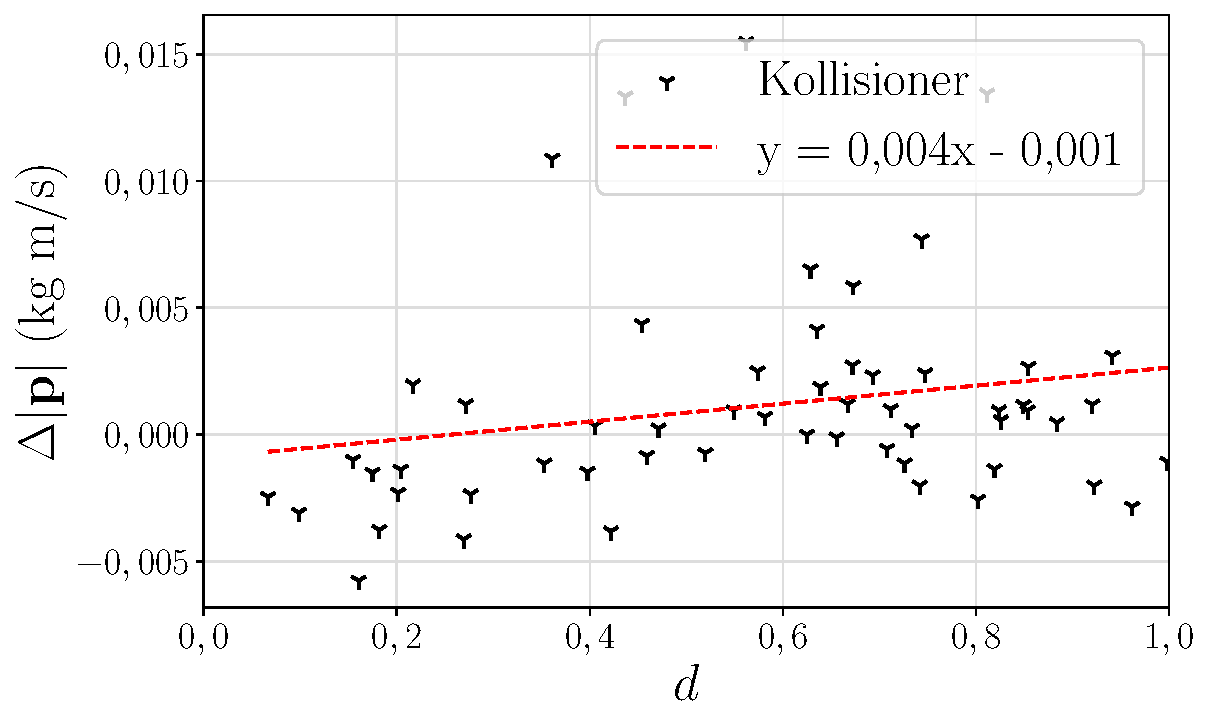
\includegraphics[width=1.2\linewidth]{images/d_deltap2.pdf} %R-squared value: 0.04484322802549928
        \caption{Rörelsemängdsbevaring med avseende på $d$. Notera mätvärdernas centrering kring 0. Regressionlinjen har ett $R^2$-värde på 0,05.}
        \label{fig:rm}
    \end{minipage} 
    \hfill
    \begin{minipage}{.45\textwidth}
        \centering
        \hspace*{-1.2cm}
        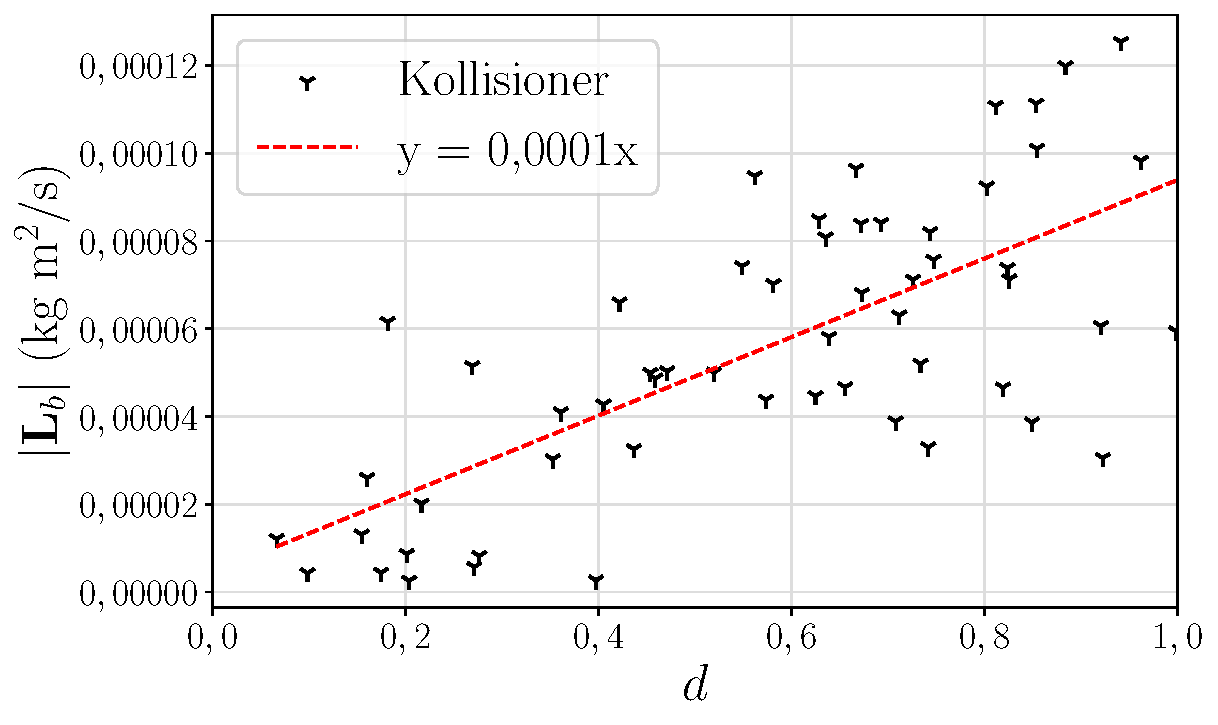
\includegraphics[width=1.2\linewidth]{images/d_lb.pdf} %R-squared value: 0.5087971703532166
        \caption{Rörelsemängdsmomentet för puck B $\mathbf{L}_b$ med avssende på $d$. Notera ökningen av rörelsemängdsmoment när d ökar. Regressionlinjen har ett $R^2$-värde på 0,51. }
        \label{fig:lb-label}
    \end{minipage}
\end{figure}

Felanalysen av resultaten består både av felfortplantningen av mätvärdena, redovisade i bilaga \ref{bil:mätos}, och referensmätningarna av objektens friktion. Referensmätningarna när varje puck och ryttare gled över ytan utan kollision visade att medelvärdet för $\Delta T$ under $\qty{0.4}{s}$ var $\SI{4.8e-4}{J}$ för ryttare A, $\SI{2.9e-4}{J}$ för ryttare B, \( \SI{3.6e-5}{J}\) för puck A och \(\SI{4.2e-5}{J}\) för puck B. 

\section{Diskussion}
Baserat på de redovisade resultaten i del 1 kan det tydligt konstateras att gummi överlag är ett mer elastiskt material jämfört med metall. Samtidigt minskar elasticitetskoefficienten \(e\) när den relativa hastigheten \(v_{\text{rel}}\) ökar för båda materialen. Med höga \(R^2\)-värden på 0,96 och 0,93 kan vi också påvisa att mätvärdena i stor utsträckning följer de anpassade funktionerna från regressionsanalysen. Det är intressant att notera hur sambandet varierar beroende på materialet. Det är svårt att entydigt förklara varför gummi uppvisar en linjär relation medan metallen följer en potensrelation enbart utifrån den presenterade teorin. En möjlig förklaring är att gummibandet har en betydligt högre elasticitetsgräns än metallen. Det innebär att det befinner sig inom sitt elastiska område inom det undersökta intervallet av \(v_{\text{rel}}\) främst förlorar energi till värme istället för att undergå plastisk deformation som metallen gör. Detta resonemang stärks av den tydliga utplaningen av \(e\) för metallen vid \(v_{\text{rel}} > \SI{0.6}{m/s}\). Det verkar som att materialet når sin elasticitetsgräns inom detta interval.

I del 2 undersöks flera aspekter av den tvådimensionella kollisionen med fokus på den initiala frågeställningen. Från mätdatan om fördelningen av kinetisk energi framgår tydligt att rotations- och translationsenergi korrelerar med \(d\). Ju längre ut mot kanten puckarna träffar varandra, desto större blir rotationsenergins andel av den totala kinetiska energin. Mätvärdena överensstämmer i hög grad med de anpassade funktionerna och ger höga \(R^2\)-värden på 0,84 och 0,86. Det observerade sambandet går dock emot det teoretiska idealfallet där impulser från puckkollisioner enbart påverkar translation eftersom impulsen skall vara riktad vinkelrätt mot kontaktytan genom masscentrum. Ytterliggare en intressant observation är att rotationsenergins andel inte överstiger cirka \(30\%\) även när \(d\) närmar sig 1. En högst trolig förklaring är förekomsten av friktion mellan kontaktytorna vid kollisionsögonblicket, vilket ger upphov till en tangentiell kraft och därmed en impuls parallellt med kontaktytan och således även ett impulsmoment. Detta impulsmoment ökar rimligen med \(d\) eftersom puck A:s rörelsemängdsvektor har en större komponent i tangentiell riktning till kollisionsytan då. Impulsmomenten förklarar sambandet med rotationsenergin, medan den tangentiella impulsen förklarar varför translationsenergin fortfarande utgör cirka \(70\%\) av den totala energin när den vinkelräta impulsen minskar för stora \(d\).

Det är också värt att notera att inte bara rotationsenergins andel ökar med \(d\), utan även det absoluta rörelsemängdsmomentet för puck B, som kan ses i figur \ref{fig:lb-label}. Dock har korrelationen ett lägre $R^2$-värde på 0,51. Svagheten i korrelationen kan möjligen förklaras av det faktum att rotationshastigheten för puck B också är beroende av rotationshastigheten för puck A innan kollisionen. Denna parameter kunde inte hållas konstant och kan sannolikt vara ansvarig för bruset i mätdatan.

Ytterligare en aspekt som analyseras är riktningen på rörelsemängdsvektorn för puck B efter stöt i förhållande till \(d\). Figur \ref{fig:px} och \ref{fig:py} visar hur puck B:s rörelsemängdsvektor delas upp i en vinkelrät och en parallell komponent i förhållande till puck A:s rörelsemängdsvektor före kollisionen. Parameteren \(p_{x'}\) mäter i grunden hur mycket puck B avviker åt sidan efter kollisionen. Även om korrelationen är svag med $R^2$-värde på 0,25 och 0,35, stödjer det den intuitiva insikten att ju längre från centrum av kollisionen puckarna kolliderar, desto mer avvikelse uppstår i sidled. Svagheten i sambandet kan troligtvis förklaras på samma sätt som för den kinetiska energin, genom impulser som verkar tangentiellt med kontaktytan och då påverkar riktningen.

Angående bevaring av rörelsemängd bekräftar resultatet teorin. I figur \ref{fig:rm} syns ingen tydlig trend och  $R^2$-värdet för regressionsanalysen är 0,05. Differensen av rörelsemängd innan och efter stöt ligger även runt 0, vilket bekräftar Newtons lagar om bevaring för slutna system.

Datainsamlingens riktighet bör även betraktas som god då mätvärdena har en relativt låg felmarginal och att energipåverkan i referensmätningarna från bordet var liten och systematisk vilket gör att påverkan på sambandet blir försumbart.

%Utifrån redovisade resultat i del 1 kan ett tydligt samband konstateras där gummi är ett överlag mer elastiskt material än metall samtidigt som $e$ avtar när $v_{\text{rel}}$ ökar för båda materialen. Med $R^2$-värde på 0,96 respektive 0,93 påvisas även att mätvärdena till hög grad följer de anpassade funktionerna som erhålls från regressionsanalysen. Dock är det intressant hur sambandet skiljer sig åt beroende på material. Anledningen till att gummi ger ett linjärt samband och metall ett potenssamband kan ej förklaras entydigt utifrån den presenterade teorin. Möjlig förklaring är att gummiband har en betydligt högre elasticitetsgräns än metallen vilket innebär att den befinner sig i sitt elastiska område för det undersökta intervallet på $v_{\text{rel}}$. Det linjära avtagandet beror således troligtvis på att gummibandet förlorar energi till värme istället för plastisk deformation som metallen. Detta resonemang styrks av ett en tydlig utplaning av $e$ för metallen kan observeras för $v_{\text{rel}}>0,6$. Bedömt uppnår materialet sin elasticitetsgräns i det intervallet.

%I del 2 undersöks flera aspekter av den tvådimensionella stöten utifrån frågeställningen. Från mätdatan om fördelningen av kinetisk energi erhålls inledningsvis ett tydligt samband att rotations- och translationsenergi beror på $d$. Desto längre ut på kanten puckarna träffar varandra ju större blir rotationsenergins andel av den totala kinetiska energin. Mätvärdena följer de anpassade funktionerna med ett relativt högt $R^2$-värde på 0,84 och 0,86. Detta samband motsäger dock det teoretiska idealfallet där impulser från kollisioner av puckar enbart påverkar translation på grund av att impulsen är riktade vinkelrät mot kontaktytan genom masscentrum. En ytterligare intressant observation är att andelen rotationsenergi inte blir större än cirka $30 \%$ även för $d$ nära 1. Högst trolig förklaring är att förekomsten av friktion mellan kontaktytorna i stötögonblicket ger upphov till en tangentiell kraft som introducerar en impuls parallell med kontaktytan och således ett impulsmoment. Impulsen och impulsmomentet ökar rimligen tillsammans med $d$ eftersom puck As rörelsemängdssvektor har en större komposant tangentiellt till kollisionsytan då. Impulsmomenten förklara isåfall sambandet med rotationsenergin och den tangentiella impulsen förklarar varför translationsenergin fortfarande utgör cirka 70 \% av totala energin när den vinkelräta impulsen blir mindre för stora $d$.

%Observation av att storheterna inte helt är bevarade enligt tidigare presenterade uttryck kommer troligtvis att göras på grund av det icke-ideala system som försöken kommer att göras i. På grund av att faktorer som både kan tillföra och tillfrånta energi till systemet kommer vara närvarande kommer till exempel stötkoeffecientens uträkning inte bli exakt. Även lufttillförseln i experimenten kan bli svår att reglera så att den skapar ett system där friktionen blir så nära noll för att behålla det slutet och beroende på alla faktorers noggrannhet samt reglerbarhet kommer överföringen divergera från 100\%.

%I den första uppställningen del 1, där relativ hastighet varieras mellan ryttarna i en en-dimensionell stöt, förväntas stötkoefficienten enligt presenterad teori idealiskt sett inte att påverkas. Dock kommer eventuella experimentella faktorer som ökade inre friktioner, rörelse i $\hat z$-led, energiförluster till ljud och värme i gummibandet påverka resultatet vid högre hastigheter. Vid lägre hastigheter kan det däremot bli intressant att studera ifall luftströmmar från skenan gör det möjligt för $e<1$ att observeras.

%I del 2 förväntas ett större $d$ enligt presenterad teori i ett idealt fall enbart påverka fördelningen mellan rörelsemängd i $\hat x$ och $\hat y$-led vid stöt. Detta på grund av att idealfallet inte tar hänsyn till friktion mellan puckarnas kontaktytor. I och med att puckarna är cirkelformade uppstår enbart radiella impulser som i sin tur enbart påverkar masscentrums translation. Genom att däremot ta hänsyn till tangentiell friktion i stöten bör stora $d$ ge upphov till större tangentiella krafter vilket i sin tur resulterar i ett impulsmoment. Det bör leda till en större rörelsemängdsmomentsöverföring som naturligt kommer bli en större andel av den ursprungliga rörelsemängden. Liknande experimentella faktorer som påverkar del 1 kommer rimligtvis även vara relevanta i del 2. Därför skall åtgärder tas för att optimera dessa faktorer så bra som möjligt för att försöka bibehålla det slutna systemet och minimera yttre faktorers påverkan.

%Resultaten av dessa experiment har potential att tillämpas inom olika fysikaliska och tekniska områden. Exempelvis kan insikterna från studien vara värdefulla både för att förbättra krocktestning i bilindustrin eller förstå kollisioner mellan himlakroppar. Detta genom att bättre förstå hur olika faktorer påverkar stötar och energiöverföring.

\section{Slutsats}
Sammanfattningsvis har detta arbete undersökt stötar i både en och två dimensioner med avseende på energi- och rörelsemängdsbevaring samt fördelningen av energi och rörelsemängd. I endimensionella stötar visade resultaten att stötkoefficienten \(e\) minskar med ökad relativ hastighet \(v_{\text{rel}}\) och att detta samband varierar beroende på materialet som används. Gummi visade sig ha en linjär relation mellan \(e\) och \(v_{\text{rel}}\), medan metallen uppvisade ett potenssamband. Detta kan troligen förklaras av skillnader i elasticitetsgräns mellan materialen.

I två-dimensionella stötar visade resultaten att fördelningen av kinetisk energi förändras beroende av kollisionspunkten \(d\). Rotationsenergins andel ökar med ökad \(d\), medan translationsenergins andel minskar. Detta samband kan troligen kopplas till friktion vid kollisionsögonblicket och resulterande tangentiella impulser. Rörelsemängden i $x'$- och $y'$-led för puck B påverkas också av \(d\), och det observerades att rotationsrörelsen i puck A påverkar rörelsemängden i puck B efter kollisionen. Dessutom ökar det absoluta rörelse-mängdsmomentet för puck B med ökad \(d\).

Dessa resultat ger insikter om hur energi- och rörelsemängdsbevaring fungerar i olika dimensioner och hur fördelningen av energi och rörelsemängd påverkas av kollisionsparametrar. Denna kunskap kan vara värdefull inom olika fysikaliska och tekniska områden, inklusive krocksimulationer och beräkning av planetsystem. Det är viktigt att notera att friktionens påverkan på kollisioner i praktiken kan vara betydande och kan ge upphov till avvikelser från ideala teoretiska modeller. 

Utvecklingsmöjligheterna för detta arbete ligger främst i att bättre förklara orsaken till de observerade sambanden och resultaten teoretiskt. I framtida undersökningar för del 1 bör fler ingående parametrar observeras. Exempelvis kan energiförluster i form av värme och ljud mätas. I del 2 kan en skjutanording användas för att säkerställa att kollisionshastighet och rotation innan stöten hålls konstant när $d$ varieras.

%

\renewcommand*{\UrlFont}{\rmfamily}
\printbibliography[heading=bibintoc]

\newpage
\appendix
\renewcommand{\thetable}{\Alph{section}.\arabic{table}}
\section{Laborationsloggbok}

I figur \ref{bil:loggbok} kan laborationsloggboken som fördes vid laborationstillfället 2023-09-23 ses.

\begin{figure}[H] 
    \centering
    \begin{subfigure}{.5\textwidth}
      \centering
      \frame{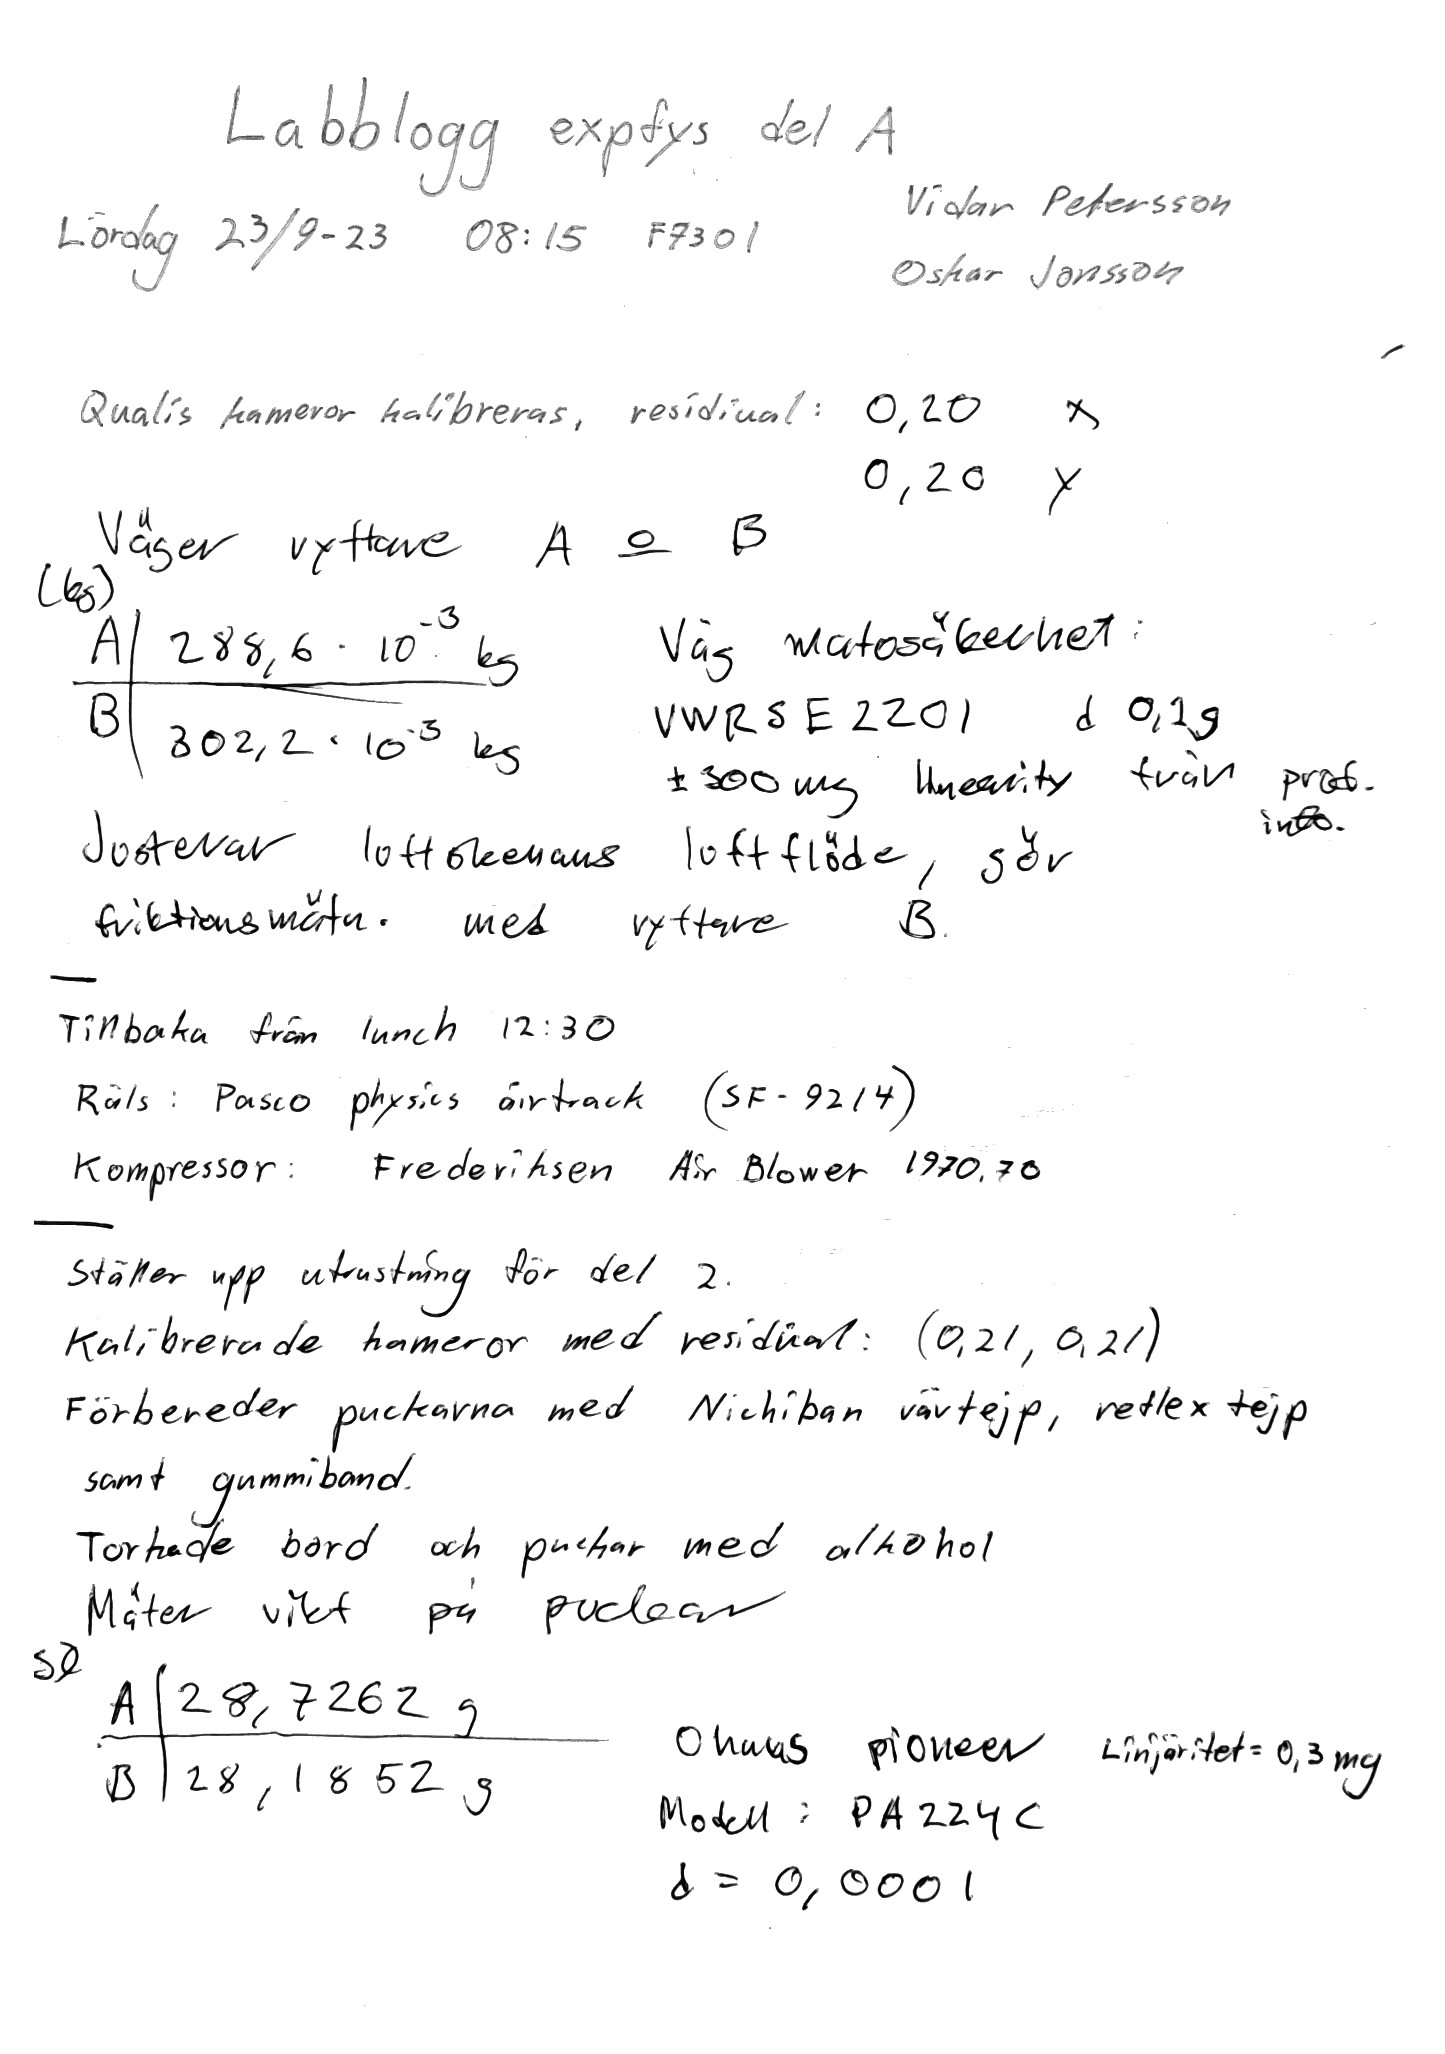
\includegraphics[width=0.85\linewidth]{bilagor/loggbok1.jpg}}
    \end{subfigure}%
    \begin{subfigure}{.5\textwidth}
      \centering
      \frame{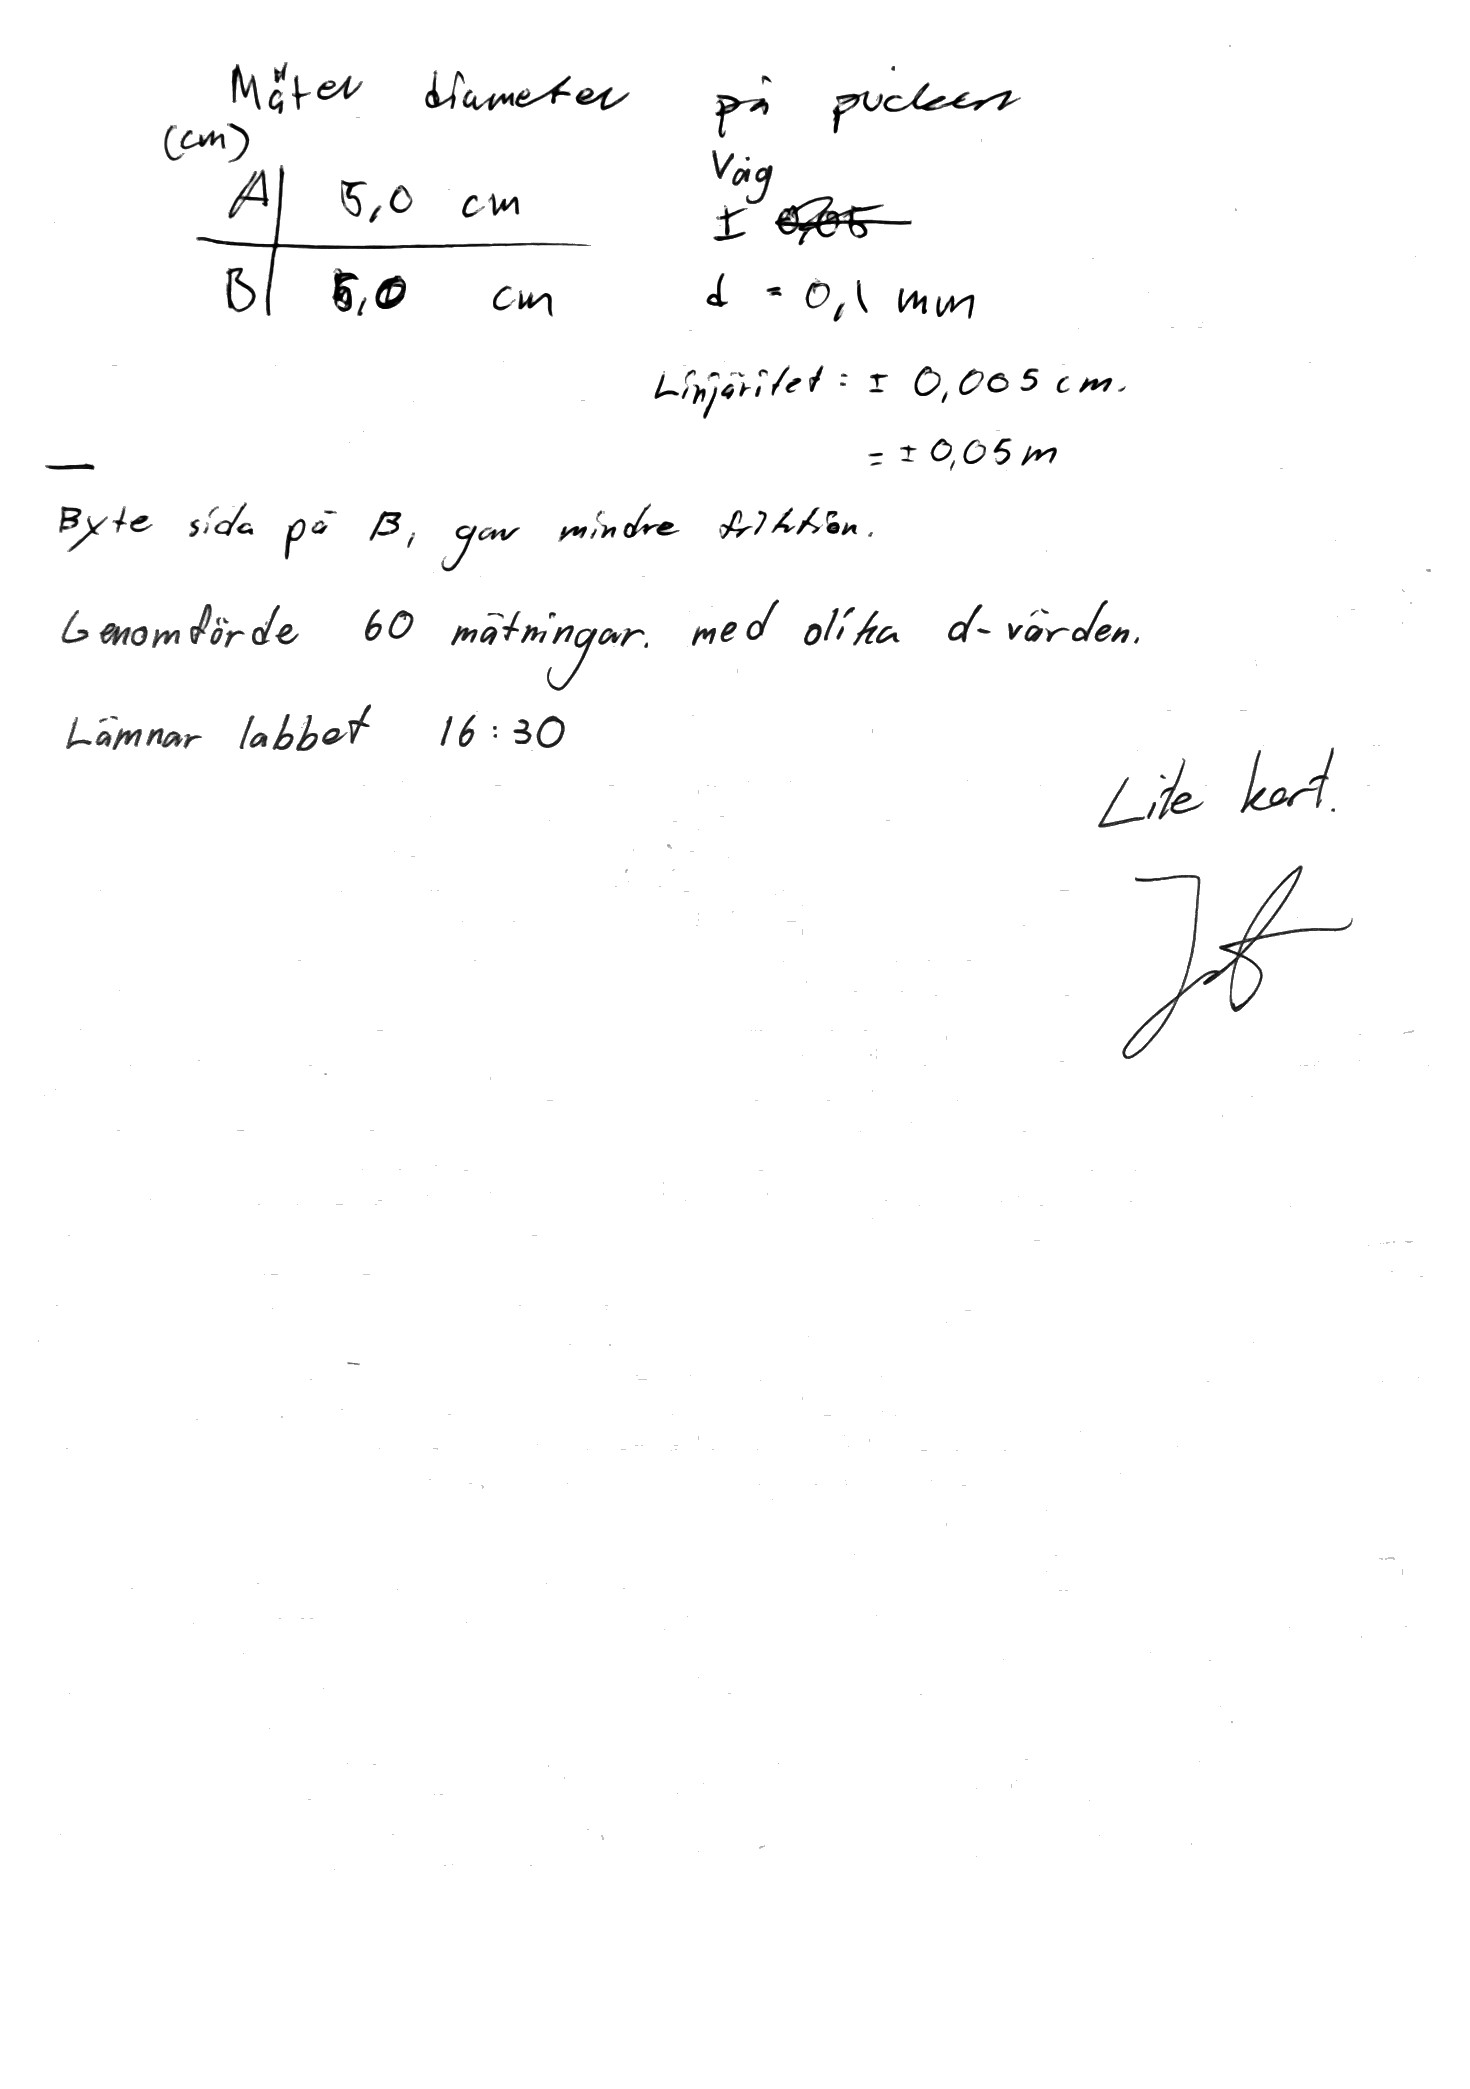
\includegraphics[width=0.85\linewidth]{bilagor/loggbok2.jpg}}
    \end{subfigure}
    \caption{Laborationsloggbok signerat av handledare.}
    \label{bil:loggbok}
\end{figure}

\section{Dataanalys}\label{bil:kod}
Denna bilaga presenterar den kod som ligger till grund för dataanalysen i arbetet. Koden använd för del 1 presenteras i lisitng \ref{lst:1main} och för del 2 i listing \ref{lst:2center_calc} och \ref{lst:2_analisys}.

\definecolor{dgray}{gray}{0.35}
\definecolor{lgray}{gray}{0.97}
\lstset{
    language=Python,
    backgroundcolor=\color{lgray},
    basicstyle=\footnotesize\ttfamily,
    commentstyle=\footnotesize\ttfamily\itshape\color{dgray},
    numberstyle=\footnotesize\ttfamily,
    numbers=left,
    frame=none,
    stepnumber=1,
    showstringspaces=false,
    tabsize=2,
    breaklines=true,
    breakatwhitespace=true,
    postbreak=\mbox{{$\hookrightarrow$}\space}
}

\lstinputlisting[
caption={Kod för dataanalys av del 1. Kod för generering av figurer har uteslutits.},
label={lst:1main},
language=Python,
]{bilagor/1_main.py}

\newpage
\lstinputlisting[
caption={Kod för numerisk beräkning av dels vilken puck mätpunkterna tillhörde och dels beräkning av masscentrums translation och rotation utifrån mätpunkternas rotation och translation i del 2.},
label={lst:2center_calc},
language=Python,
]{bilagor/2_center_calc.py}

\newpage
\lstinputlisting[
caption={Kod för numerisk beräkning av puckarnas tillstånd innan och efter kollision. Kod för generering av figurer har uteslutits.},
label={lst:2_analisys},
language=Python,
]{bilagor/2_analisys.py}


\section{Mätvärden} \label{bil:mätning}

\begin{table}[H]
\centering
\caption{Uppmätta konstanter av ryttarna i del 1.}
\label{tab:prop1}
\begin{tabular}{@{}ll@{}}
\toprule
Objekt    & Massa                                 \\ \midrule
Ryttare A  & $\SI{0.2886(1)}{kg}$                 \\
Ryttare B med gummiband& $\qty{0.3022(1)}{kg}$  \\
Ryttare B utan gummiband& $\qty{0.2982(1)}{kg}$ \\ \bottomrule
\end{tabular}
\end{table}

\begin{table}[H]
\centering
\caption{Uppmätta och beräknade konstanter av puckarna 2.}
\label{tab:prop2}
\begin{tabular}{@{}lll@{}}
\toprule
Objekt    & Massa                   & Radie             \\ \midrule
Puck A    & $\qty{0.0287262(1)}{kg}$   & $\qty{0.025(0.0005)}{m}$          \\
Puck B    & $\qty{0.0281852(1)}{kg}$   & $\qty{0.025(0.0005)}{m}$          \\ \bottomrule
\end{tabular}
\end{table}

\section{Mätutrustning} \label{bil:mätutr.}
\begin{table}[H]
\centering
\caption{Översikt över den mätutrustning som användes för att mäta objekten.}
\label{tab:mätutr.}
\begin{tabular}{@{}lllll@{}}
\toprule
Instrumenttyp & Modellnamn     & Mätte         & Upplösning        & Linjäritet            \\ \midrule
Våg           & VWR   & Ryttarna & $\SI{e-4}{kg}$    & $\SI{\pm 3e-4}{kg}$   \\
& (SE2201)   & &     &    \\
Våg           & Ohaus Pioneer & Puckarna    & $\SI{e-7}{kg}$    & $\qty{\pm 3e-7}{kg}$  \\
           & (PA224C) & &  &   \\
Skjutmått     & Okänd         & Puckarna    & $\qty{5e-5}{m}$   & -                     \\ 
Motion capture & Qualisys Oqus 300 & Alla           & $\qty{e-6}{m}$    & -                     \\ \bottomrule
\end{tabular}
\end{table}

\section{Mätosäkerhet}\label{bil:mätos}
För storheterna i figurerna beräknas i denna bilaga deras mätosäkerhet med hjälp av insamlade värden på mätutrustning samt medelvärdet av samtlig insamlad data för att få fram felfortplanAtningen för varje enskild storhet. Detta sker enligt formeln
\begin{equation}\nonumber
\sigma_{f}^2 = \left(\frac{\partial f}{\partial a}\right)\sigma_{a}^2 + \left(\frac{\partial f}{\partial b}\right)\sigma_{b}^2 + \left(\frac{\partial f}{\partial c}\right)\sigma_{c}^2 + ...
\end{equation}
där funktionen $f = f(a,b,c,...)$ är uppbygd av flera variabler med ett eget osäkerhetsvärde.

\begin{table}[H]
\centering
\caption{Beräknad felfortplantning för storheter.}
\label{tab:felfort}
\begin{tabular}{@{}lll@{}}
\toprule
Storhet    & Felfortplatning                             \\ \midrule
$e$             &  $4,56\%$                                     \\
$v_{\text{rel}}$       &  $1,23\%$                                     \\
$T$             &  $4,32\%$                                     \\
$d$             &  $5,12\%$                                     \\
$\mathbf{p}$    &  $3,45\%$                                     \\
$\mathbf{L}$    &  $3,81\%$                                     \\ \bottomrule
                                                
\end{tabular}
\end{table}

\section{Peer-granskning}
\textbf{Sammanfattning av återkoppling från grupp 13: } Stavfel och syftningsfel i inledning, metod och teori. 

\textbf{Vidtagna åtgärder: } Korrigerade stavfel och syftningsfel i inledning, metod och teori.

\end{document}
